Vamos a hacer uso de la implementación mediante un \textbf{vector de posiciones relativas} ya que estos son muy útiles y eficientes cuando trabajamos con árboles completos.

La parte privada del TAD quedaría:
\begin{verbatim}
template <typename T> class Apo{
  public:
    //Métodos vistos en la Especificación del TAD.
  private:
    typedef size_t nodo; //Indice del vector.
    size_t maxNodos; //Tamaño del vector (árbol).
    size_t numNodos; //Número de nodos (último nodo del árbol)
    T* nodos; //Vector de nodos
    //Métodos privados de la clase
    nodo padre(nodo n)const;
    nodo hIzq(nodo n)const;
    nodo hDer(nodo n)const;
    void hundir(nodo n);
    void floar(nodo n);
};
\end{verbatim}
\newpage
\subsection*{Inserción de elementos en un APO}
\begin{figure}[h]
  \begin{center}
    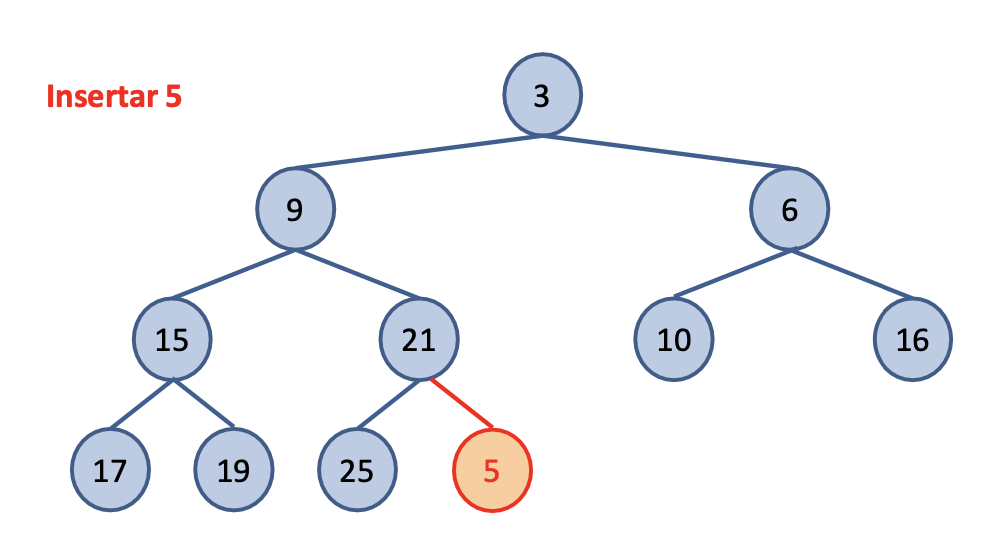
\includegraphics[width=0.7\textwidth]{assets/apo2.png}
  \end{center}
  \caption{Ejemplo de inserción 1.}
\end{figure}
Queremos insertar el valor `5' en nuestro APO el cual no está vacío, por tanto, vamos a insertarlo en la última posición del vector de posiciones relativas que equivale al hijo derecho del nodo con valor `21'. A continuación vamos flotando dicho nodo hasta que se cumpla la propiedad de ordenación.
\begin{figure}[h]
  \begin{center}
    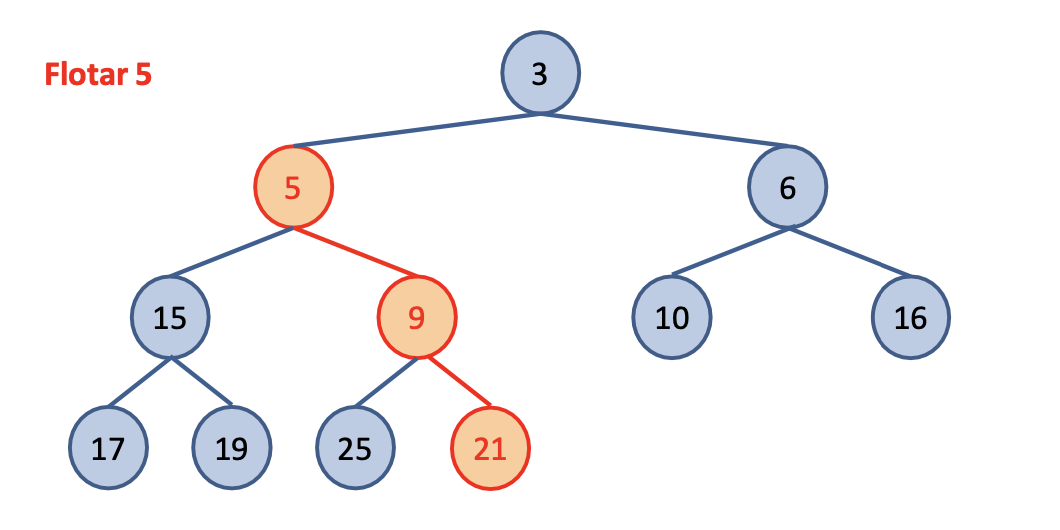
\includegraphics[width=0.7\textwidth]{assets/apo3.png}
  \end{center}
  \caption{Ejemplo de inserción 2.}
\end{figure}
Tenemos como resultado que el nodo con valor `5' es el nuevo hijo izquierdo del nodo raíz, y por tanto, vemos que todos los nodos están ordenados.
\subsubsection*{Código de Inserción y Flotar}

\underbar{Código de insertar:}
  \begin{verbatim}
template <typename T> 
void Apo<T>::insertar(const T& e){
  assert(numNodos < maxNodos);
  //insertamos en la última posición.
  nodos[numNodos] = e; 
  //Llamamos al método flotar
  if(numNodos > 1)
    flotar(numNodos-1);
}
  \end{verbatim}
\underbar{Código de flotar:}
\begin{verbatim}
template <typename T>
void Apo<T>::flotar(nodo n){
  //Guardamos el contenido del nodo
  T e = nodos[n];
  //recorremos los nodos intercambiandolos
  while(n>0 && e < nodos[padre(n)]){
    nodos[n] = nodos[padre(n)];
    n = padre(n);
  }
  nodos[n] = e;
}
\end{verbatim}

\subsection*{Eliminación de elementos en un APO}
\begin{figure}[h]
  \begin{center}
    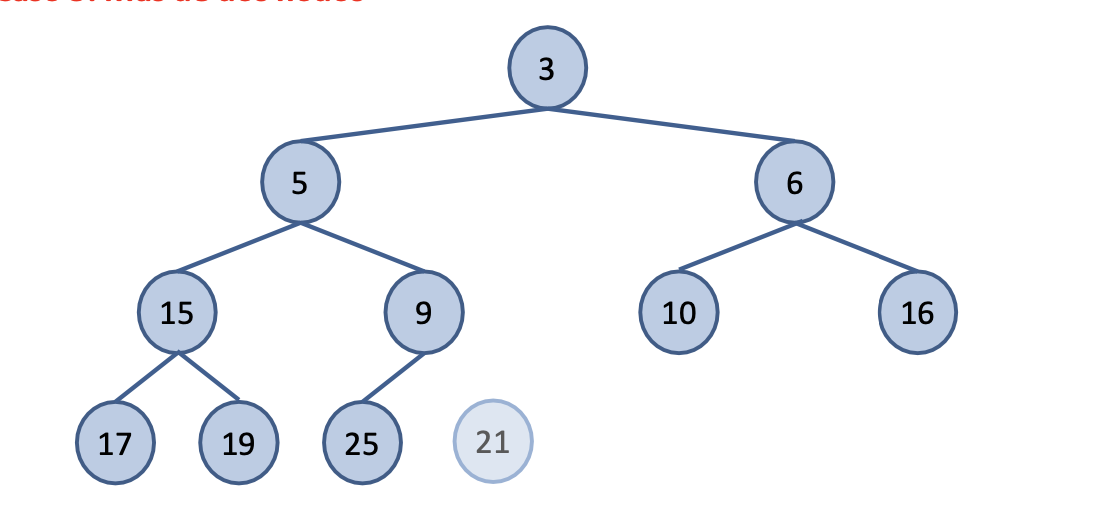
\includegraphics[width=0.7\textwidth]{assets/apo4.png}
  \end{center}
\end{figure}

Vemos que queremos realizar la eliminación del nodo raíz con contenido `3', por tanto, el último nodo del árbol `21', ocupará la posición del nodo raíz sobrescribiendo su contenido y por ende tendremos que hundir dicho nodo para que el APO siga ordenado.
\begin{figure}[h]
  \begin{center}
    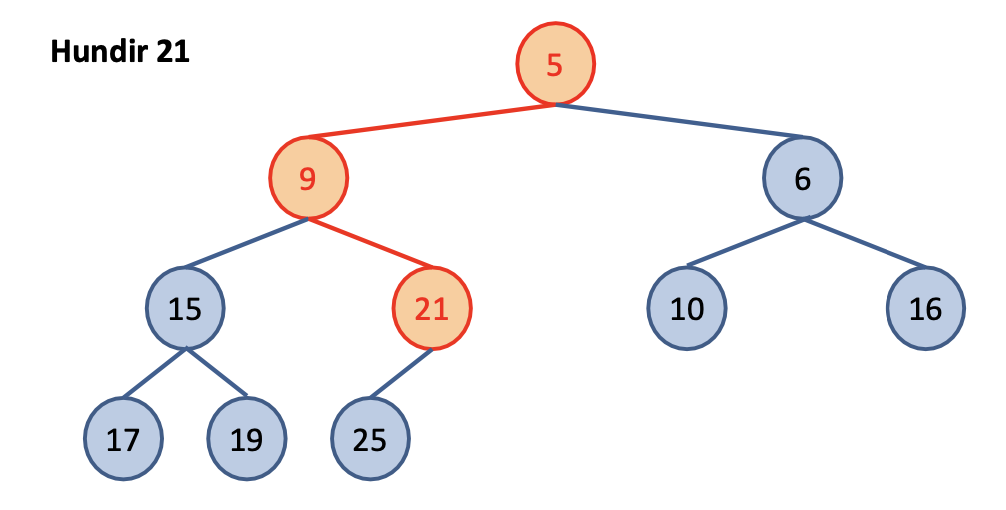
\includegraphics[width=0.7\textwidth]{assets/apo5.png}
  \end{center}
\end{figure}

COmo resultado tenemos que el nodo con valor `21' ahora es padre del nodo con valor `25' y el nuevo nodo raíz es el nodo con valor `5' que previamente era el hijo izquierdo del nodo con valor `3' (la raíz anterior).

\underbar{Código de suprimir:}
\begin{verbatim}
template <typename T>
void Apo<T>::suprimir(){
  assert(numNodos > 0);
  if(--numNodos > 0){
    nodos[0]=nodos[numNodos];
    if(numNodos > 1)
      hundir(0);
  }
}
\end{verbatim}
\underbar{Código de hundir:}\\
\begin{verbatim}
template <typename T>
void Apo<T>::hundir(nodo n){
	bool fin = false;
	T e = nodos[i];
	while (hIzq(i) < numNodos && !fin){
	nodo hMin;
	if (hDer(i) < numNodos && nodos[hDer(i)] 
      < nodos[hIzq(i)])
	hMin = hDer(i);
	else
	hMin = hIzq(i);
	if (nodos[hMin] < e){
	nodos[i] = nodos[hMin];
	i = hMin;
}
	else
	  fin = true;
}
	nodos[i] = e;
}
\end{verbatim}